Preden se lahko izdela primerjavo podatkovnih struktur je potrebno predstaviti okolje, v katerem bo izdelana primerjava, metoda uporabljena za izdelavo testnih primerov ter sami testni primeri, ki bodo uporabljeni za izdelavo primerjave. V tem podpoglavju bodo prvo predstavljeni testni primeri, za tem bo predstavljena uporabljena testna metoda ter na koncu bo predstavljen stroj in operacijski sistem, ki je uporabljen za izdelavo testiranja. 

\subsection{Testni primeri}

Empirična primerjava je bila izdelana nad dvema vhodnima besedama, ki sta prikazani v Tabeli \ref{tab:besedila}. Prva testirana beseda je daljša DNK sekvenca \cite{podatki}, ki je zlepek različnih DNK sekvenc in je označena kot \DNK. Izbrana je bila kot primer vhodne besede, uporabljene v bioinformatiki. Ta vhodna beseda je bila predhodno uporabljena za testiranje implementacije kompaktnega priponskega drevesa od Välimäki idr. \cite{Valimaki2007}. Abeceda $\Sigma$ besede \DNK sestoji iz nukleotidov, ki jih označimo z črkami A, C, T in G. Zato smo se odloči, da nukleotide predstavimo kot 7 bitne ASCII znake.

\begin{table}[htb]
    \caption{Primerjava besedil, ki smo jih uporabili za primerjavo različnih indeksov besed}
    \label{tab:besedila}
    \centering
    \begin{tabular}{rccc}
        Ime testne besede& Število znakov & Velikost abecede & Velikost na disku \\
        &  &   & [MB]\\
         \hline
        Ivan Cankar, Na klancu \cite{podatkiNaKlancu}& 317803 & 53 & $25,851$ \\
        DNK sekvenca \cite{podatki}&  52428800& 5 & $26,767$ \\
    \end{tabular}    
\end{table}

Druga testirana beseda je Cankarjev kratki roman Na klancu \cite{podatkiNaKlancu}, ki je označen kot \NK. Roman je bil izbran, saj predstavlja tipično vhodno besedo v naravnem jeziku, ki je v tem primeru slovenščina. Abeceda $\Sigma$ besed \NK sestoji iz črk slovenske abecede (velikih in malih), presledkov in ločil. Ker smo se odločili, da predstavimo \DNK z ASCII znaki, je bilo potrebno \NK v ASCII. Zato so bili vsi ne ASCII znaki odstranjeni oziroma zamenjani z ASCII alternativami. Na primer znak, ki predstavlja '...', je bil zamenjan s tremi pikami, vse črke z naglasi (kot so strešice, ostrivci ter drugi) so bile zamenjani z osnovnim znakom, zato š postane s in é postane e. Odstranjene so bile tudi vse prazne vrstice ter ločila poglavij, ki so bila označena z '***', saj le-te ne vplivajo na vsebino besedila. Odstranjeni so bili tudi vsi simboli, ki niso vidni bralcu, prisotni v besedilu. Na ta način se je začetno besedilo znižalo iz dolžine 319843 znakov na 317803.

\paragraph{Podaljševanje besedila.}

V drugem stolpcu Tabele \ref{tab:besedila} so prikazane dolžine besed, ki so bila uporabljena za testiranje. Pri tem se opazi, da so beseda \NK je krajša od 1024500 znakov, ki so potrebni za izgradnjo indeksov in za izdelavo vzorcev testiranja. Zato jo je bilo potrebno podaljšati. Ker je malo verjetno, da se vhodna beseda ponovi $k$-krat, dokler ne doseže primerne velikosti, predvsem v naravnem jeziku, je bila uporabljena bolj napredna metoda podaljševanja besedila. Metoda vzame manjše podnize besedila ter naredi stik med začetno besedo in podnizom. Tako dobljena beseda je bolj verjetna, saj je večja verjetnost, da se manjši deli besede ponovijo za razliko od celotne besede. Predlagana metoda podaljševanja besede je prikazana v Algoritmu \ref{alg:Konkatenacija}. Pri tem metoda predpostavi, da je beseda dolga vsaj $3000$ znakov. Ta metoda je primerna za podaljševanje daljših besed, sicer pa je možno metodi spremeniti parameter $i$ in tako prilagoditi metodo drugim besedam.


\begin{algorithm}[htb]

\Vhod{Vhodna beseda $T$, velikost $s_{max}$}
\Izhod{Besedilo $T_0$}
\caption{Metoda podaljševanja vhodne besede}\label{alg:Konkatenacija}
{
    {$T_0\leftarrow T$}

    {$i\leftarrow 500$}
    
    \While{$|T_0| < s_{max}$}{
        
        {$T_0\leftarrow T_0\cdot T[i:6i]$}
        
        
        {$i\leftarrow i+500$}

        \While{$6i>|T|$}{$i=i/4$}
        
    }
    \Vrni{$T_0[1:s_{max}]$}    
    
}
\end{algorithm}

Predlagana metoda podaljša besedo na velikost $s_{max}$. Ta velikost je lahko dolžina najdaljše besede ali pa je poljubna vrednost, bodisi manjša od dolžine največje besede bodisi večja. Če je beseda daljša od velikosti $s_{max}<|T|$, bo predlagana metoda skrajšala besedo na $|T_0|=s_{max}$. Za potrebe testiranja smo se odločili, da je $s_{max}=25000000$, kar je več kot zadostna dolžina.

\subsection{Metoda testiranja}
Strukturna primerjava je prikazana s psevdokodo na Algoritmu \ref{alg:metodaTest}. Vsak test v primerjavi se je izvedel petkrat, da se je zmanjšal vpliv drugih procesov na rezultate testiranja. Iz psevdokode opazimo, da je bila primerjava poizvedb storjena za poizvedbo $\Prisotnost{T}{P}$, saj je pogosto vprašanje v biologiji prisotnost gena (vzorcev $P$) v DNK sekvenci (vhodna beseda $T$), ne pa natančen položaj tega gena ali števila ponovitev gena v DNK sekvenci. Poizvedba je bila izdelana za vzorce velikosti 5, 50, 500 in $\log{|T|}$ (na psevdokodi $\log{i}$ v vrstici \ref{alg_line:log}). Rezultati testiranja so bili shranjeni v seznamu in vsaka rezultat hrani sledeče podatke: tip podatkovne strukture, velikost vhodne besede, čas gradnje, čas iskanja vzorca dolžine 5, čas iskanja vzorca dolžine 50, čas iskanja vzorca dolžine 500, čas iskanja vzorca dolžine $\log{|T|}$ ter velikost podatkovne strukture. Velikost bo dodana iz podatkov pridobljenih s pomnilniškim profilerjem (angl. \textit{memory profiler}), zato je ni navedene v vrstici \ref{alg_line:shrani}. 

\begin{algorithm}[htb]

\Vhod{Vhodna beseda $T$, število znakov v najdaljšem testiranem nizu $i_{max}$}
\Izhod{Tabela z izračunanimi časi}
\caption{Psevdokoda primerjave indeksov vhodne besede $T$}\label{alg:metodaTest}
{
    {$i \leftarrow 500$}
    
    \Dokler{$i \le i_{max}$}{

        \Za{$S\in\{ST, SA, SA+LCP, CST\}$}{
            \Za{$k=1,\dots,5$}{
                {$\textit{start}\leftarrow \textit{čas}()$}  \Comment*[r]{\v{}\v{}\v{} testiranje}

                {$\textit{Izgradi}(S,T[1:i-1]\cdot\$)$}

                {$\textit{konec}\leftarrow \textit{čas}()$} \Comment*[r]{\^{}\^{}\^{} testiranje}

                {$t_{Izg}\leftarrow \textit{konec} - \textit{start}$}

                \Za{$j\in\{5, 50, 500 \}$}{
                    {$\textit{start}\leftarrow \textit{čas}()$} \Comment*[r]{vvv testiranje}

                    {$\Prisotnost{S}{T[i:i+j]}$}

                    {$\textit{konec}\leftarrow \textit{čas}()$} \Comment*[r]{\^{}\^{}\^{} testiranje}

                    {$t_{j} \leftarrow \textit{konec} - \textit{start}$}
                }

                {$j\leftarrow \log{i}$\label{alg_line:log}}

                {$\textit{start}\leftarrow \textit{čas}()$} \Comment*[r]{\v{}\v{}\v{} testiranje}

                {$\Prisotnost{S}{T[i:i+j]}$}

                {$\textit{konec}\leftarrow \textit{čas}()$} \Comment*[r]{\^{}\^{}\^{} testiranje}

                

                {$t_{log} \leftarrow \textit{konec} - \textit{start}$}

                {$\textit{Shrani}(S,i,t_{Izg},t_{5},t_{50},t_{500},t_{log}$)\label{alg_line:shrani}}

                {$\textit{Izbriši}(S)$}
            }
        }        
        
        {$i \leftarrow 2\cdot i$}
        
    } 
    
}
\end{algorithm}

\subsection{Stroj in operacijski sistem}
Za izdelavo primerjav podatkovnih struktur bo uporabljen računalnik s procesorjem Intel Core i3 5005U z dvema jedroma in štirimi nitmi ter s taktom $1,9$ GHz. Računalnik ima na razpolago 4 GB delovnega pomnilnika, od katerega je ob zagonu zasedenega $1,35$ GB z operacijskim sistemom ter emulatorjem terminala (angl. \textit{terminal emulator}). Poleg delovnega pomnilnika ima računalnik še $8$ GB Swap razdelka na trdem disku, ki je namenjen shranjevanju neuporabljenih pomnilniških strani v primeru prezasedenega delovnega pomnilnika in posledično sproščanju le tega. Operacijski sistem računalnika je Fedora 42 in uporabljen Linux kernel je 6.14.11-300.

Primerjava je izdelana v programskem jeziku C++\footnote{Koda je dostopna na povezavi \url{https://github.com/GioGiou/MagisterskaNalogaKoda}.}. Zato se časi, potrebni za izgradnjo struktur ter poizvedb v njih, izmerijo z beleženjem trenutnega časa pred začetkom, ki ga shranimo v spremenljivko \verb|start|, in po koncu operacije, ki ga shranimo v spremenljivko \verb|stop|. Meritve so implementirane s funkcijo \verb|high_resolution_clock::now()|, ki je del standardne knjižnice programskega jezika C++ in vrne natančen čas trenutka, v katerem je funkcija izvedena. Čas izvajanja se lahko naračuna kot razlika med časom ob koncu izvajanja in časom ob začetku izvajanja operacije, kar se v C++ stori s funkcijo \verb|duration_cast<nanoseconds>(stop - start)| \verb|.count()|. Za izgradnjo podatkovnih struktur bodo uporabljene sledeče knjižnice: za priponsko drevo je uporabljena implementacija iz knjižnice \cite{ganeshk13}, za kompaktna priponska drevesa je uporabjena implementacija iz knjižnice SDSL \cite{gbmp2014sea} in za priponska polja pa je uporabljena implementacija iz knjižnice \cite{Grebnov2025}. Le-ta zgradi priponsko polje v $O(n)$ časa z algoritmom, ki sta ga predstavila Timoshevskaya in Feng \cite{Timoshevskaya2014}. Algoritem je izboljšava predhodno predstavljenega algoritma od Ko in Aluru \cite{Ko2005}. Pri tem pa je uporabljena različica LCP polja imenovana $Q-LCP$ polje, ki je bila predstavljena v podpoglavju \ref{sec:SAPoizvedbe}.
%Knjižnica \cite{Grebnov2025} sicer podpira izgradnjo LCP strukture, ki je bila predstavljena v podpoglavju \ref{sec:STsimulacija}, ampak nima dodatne podatkovne strukture Fischer-Heun za operacijo $rmq$ v konstantnem času \cite{Fischer2007}.

Poleg časovne zahtevnosti gradnje in poizvedb v podatkovnih strukturah nas zanima, koliko prostora zasede posamična podatkovna struktura  na delovnem pomnilniku. In sicer nas zanima največji zaseden prostor v času izgradnje posamične podatkovne strukture. Le-ta bo izmerjen z uporabo pomnilniškega profilerja. Uporabljen bo pomnilniški profiler Bytehound \cite{Bytehound2024}, saj omogoča grafični prikaz porabe pomnilnika v času izvajanja programa.

Ker je primerjava izdelana v C++, je potrebno kodo prevesti v izvršljivo datoteko. To je strojeno s prevajalnikom GCC 15.1.1. Program je bil preveden s sledečim ukazom:
\begin{lstlisting}[language=bash]
    g++ -std=c++11 -O3 -DNDEBUG -I ./include -L ./lib // 
    main.cpp -o main -lsdsl -ldivsufsort //
    -ldivsufsort64 -lsuffix -lsais
\end{lstlisting}
Pri prevajanju programa je uporabljenih nekaj zastavic, ki določajo vrednosti parametrov prevajalnika. Večina zastavic je vezana na uvažanje knjižnic v prevajanje, in sicer \verb|-I ./include| nastavi pot do zaglavnih datotek (angl. \textit{header files}), \verb|-L ./lib| nastavi pot do strojne kode knjižnice ter zastavice \verb|-lsdsl|, \verb|-ldivsufsort|, \verb|-ldivsufsort64|,  \verb|-lsais| in \verb|-lsuffix| uvozijo potrebne knjižnice za izgradnjo izvršljive datoteke.
Zastavica \verb|-O3| določa nivo optimizacije izvršljive datoteke na nivo 3, ki je bil izbran, saj je uporabljen za prevajanje prve implementacije kompaktnega priponskega drevesa \cite{Valimaki2007}. Ker se uporablja profiler, je potrebo pred začetkom testiranja indeksov besed zagnati tudi profiler, kar je storjeno z ukazom:
\begin{lstlisting}[language=bash]
    export MEMORY_PROFILER_LOG=info
    LD_PRELOAD=~/bytehound/libbytehound.so ./main // 
    ./test/NaKlancu.txt 
\end{lstlisting}
Prva vrstica ukaza določa stopnjo profiliranja, ki ima v tem primeru vrednost \verb|info|, ter se jo shrani v sistemsko spremenljivko \verb|MEMORY_PROFILER_LOG|. Naslednja vrstica pa požene program ter se poda kot prvi parameter ime datoteke s testnimi podatki. Zgornji ukaz prikaže primer za vhodno besedilo Na klancu. S spremenljivko \verb|LD_PRELOAD| je določen deljeni objekt (angl. \textit{shared object}), ki je izvršen pred začetkom programa. V primeru testiranja je deljeni objekt profiler, kar mu omogoča dostop do programa in lažje beleženje zasedenega delovnega spomina.

Dolžina najdaljše vhodne besed $i_{max}$ je bila sprva nastavljena na 4000000 znakov. Med testiranjem priponskega drevesa besede dolžine 2048000 znakov se je opazilo, da čas, potreben za izgradnjo prvega priponskega drevesa, presega 5 minut. Po petih minutah od začetka gradnje drevesa lahko opazimo, da je delovni pomnilnik skoraj v celoti zaseden ter je Swap razdelek zaseden že s 6 GB pomnilniški strani. Pri tem je računalnik neodziven in proces je v neprekinjenem spanju (angl. \textit{Uninterruptible sleep} ali stanje D). Na Sliki \ref{fig:6GB} je prikazan upravljalnik opravil Htop v času izgradnje priponskega drevesa za besedo dolžine 2048000 znakov. Proces v modri vrstici predstavlja program za testiranje časa izgradnje in poizvedb ter prostorske zahtevnosti indeksov besed. V stolpcu, označenim S (Stanje ali angl. \textit{Status}), je vidno, da je je stanje procesa označeno kot D, ker je proces v neprekinjenem spanju. Po več kot 5 minutah od začetka gradnje priponskega drevesa za besedo dolžine 2048000 znakov smo se odločili, da se proces ubije. Posledično se je znižala velikost besede za izgradnjo zadnjega indeksa na 1024000 znakov. Med testiranjem smo opazili tudi, da se $LCP$ polje ne zgradi za besede dolžine 1024000 znakov, zato smo se odločil, da se ta test v tem koraku izpusti.

\begin{figure}[tb]
    \centering
    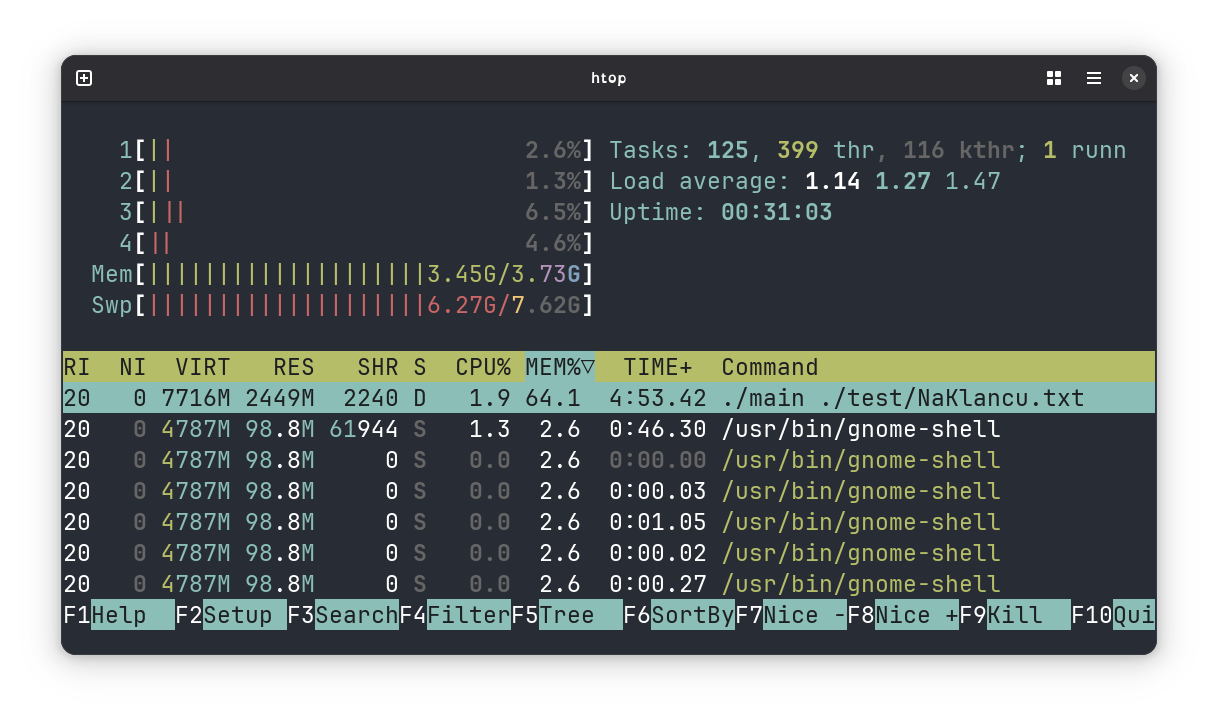
\includegraphics[width=\textwidth]{Slike/Zaslonski posnetek 2025-06-23 22-53-56.png}

    \caption{Posnetek zaslona upravljalnika opravil Htop med izgradnjo priponskega drevesa za besedilo dolžine 2048000 znakov.} 
    \label{fig:6GB}
\end{figure}



